\documentclass[a4paper,12pt]{article}

% Font
\usepackage[T1]{fontenc}
\usepackage{gentium}

% Math packages
\usepackage{amsmath}
\usepackage{amsfonts}
\usepackage{amssymb}
\usepackage{amsthm}
\usepackage{bm}

% Define symbol shortcuts
\newcommand{\cc}{\mathcal{C}}
\newcommand{\dd}{\mathcal{D}}
\newcommand{\hh}{\mathcal{H}}
\newcommand{\xx}{{\bm x}}
\newcommand{\yy}{{\bm y}}

% Math environment
\newtheorem*{thm}{Theorem}

% Better list management:
% - vertical spacing in lists
% - items in lists start with dash not bullet point.
\usepackage{enumitem}
\setlist{label=\textemdash,
  itemsep=0pt, topsep=3pt, partopsep=0pt}

% Include graphics
\usepackage{graphicx}
\usepackage{subcaption}

% Page format 
\usepackage[top=2cm,left=2cm,right=2cm,bottom=2cm]{geometry}

\begin{document}
%%% HEADER
\raisebox{0.6in}[0in]{\makebox[\textwidth][r]{\it Unproofed version }}
\vspace{-0.7in}

\begin{center}
\bf\large MA2823: Foundations of Machine Learning \\
Chapter 6: Regularized Linear Regression
\end{center}

\noindent
Lecturer: Chlo\'e-Agathe Azencott   
\hfill
Scribe: Adrien Galamez \\
\null \hfill Paul Magon de la Villehuchet


\noindent
\rule{\textwidth}{1pt}

\medskip

In this chapter we will see:
\begin{itemize}
\item what is regularization;
\item how to use regularization as a means to control model complexity;
\item several forms of regularizing linear regression models.
\end{itemize}

\section{Regression setting}
\subsection{Large $p$, small $n$}
This section is a reminder of the context in which we work. We consider a dataset that has $p$ features and $n$ samples. Thus, we're working with a data matrix $X$ that have $n$ rows and $p$ columns. The outcome vector $y$ describes the quantity we want to predict. The goal of the linear regression model is to approximate $y$ as a linear combination of $X$.
\begin{figure}[!h]
\centerline{
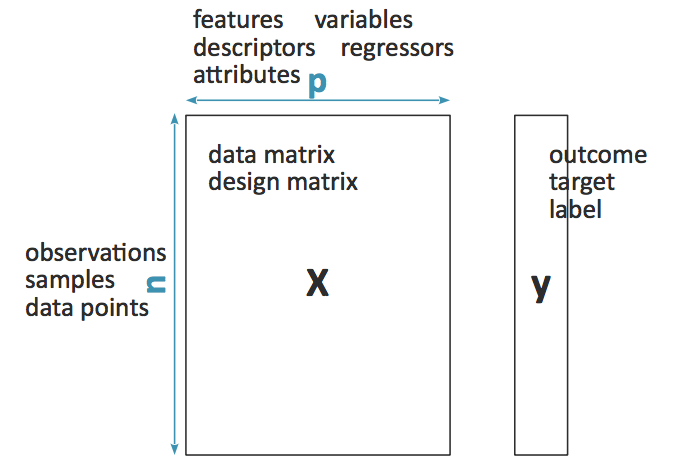
\includegraphics[scale = 0.3]{figures/RegressionSettings.png}}
\caption{Figure illustrating the dimensions of the data matrix and the outcome vector.}
\label{DataMatrix}
\end{figure}

On the Figure \ref{DataMatrix}, we can see that the data matrix is taller than it is wide ($p < n$). This is a  common shape. But, conversed settings can also appear. 

This configuration is called large $p$, small $n$. The data matrix is wider than it is tall. This is the kind of settings we have in genetics and neuroimaging: we have many more descriptors than we have data points. For instance, in genetics, a data set can gather informations for thousands of genes as this information is easy to access. Yet, as each row holds data gathered on a patient, we have at best hundreds of patients. Thus, we have a tall but not wide data matrix. In neuroimaging, brain images are big objets, typically thousands pixels or voxels (3D images). Yet, as brainscans are costly to obtain, we repeat the process on thousands of patient. Thus, we'll have more features than observations. In this configuration, we are going to need regularization.

\subsection{Linear regression}
\subsubsection{Pro and cons of least-squares fit}
Linear regression is aimed at approximating $y$ as a linear combination of X. In the previous chapter, we said that, if we're doing a least-squares fit (which is equivalent to Maximum Likelihood estimation under the assumption of Gaussian noise), we obtain this solution
\begin{equation}
\hat{\beta} = \arg\min_{\beta} (y-X\beta)^{T} (y-X\beta) = (X^T X)^{-1} X^T y.
\label{LR}
\end{equation}
This solution is uniquely defined when $X^T X$ is invertible, hence when $X$ has a full column rank. As $X$ is an $n \times p$ matrix, if $p$ is larger than $n$ (as in the large $p$, small $n$ configuration), $X$ can not be inverted.

This fit has several advantages.
\begin{itemize}
\item The predicted vector $\hat{\beta}$ is unbiased ($\mathbb{E}[\hat{\beta}]= \beta$).
\item If we're restricting to unbiased estimators, minimum mean squared error implies minimum variance.
\item This fit gives an explicit solution (Equation \ref{LR}).
\item If $n \gg p$, the computational time is linear in the number of samples. Indeed, the computational time is $O(\underbrace{np^2}_{\text{compute } X^T X}+\underbrace{p^3}_{\text{invert } X^T X})$. 
\end{itemize}

Yet, this fit has also some drawbacks.
\begin{itemize}
\item Correlated variable leads to high variance of the estimator.
\item Prediction error increases linearly as a function of $p$.
\item The solution is hard to interpret when $p$ is large as shown in the section \ref{LargeP}.
\end{itemize}

\subsubsection{When $p$ in larger than $n$}
\label{LargeP}
When $X^T X$ is not invertible, we still have ways to find $\hat{\beta}$. In this case, we can use the pseudo-inverse of $X$. We can also use numerical methods to solve a linear system of $p$ equations such as gradient descent (minimizing a convexe function), Gaussian elimination or LU decomposition.
On the Figure \ref{LRPseudoInverse}, we can compare the predicted coefficient (thanks to a linear regression using pseudo-inverse) and the true coefficient when $p = 1000$ and $n = 10$. So, we're in the case of the large $p$, small $n$ configuration. In fact, the outcome vector $y$ was created by a linear combination of the data-matrix $X$ using the weights shown on the left hand graph. 

The objectif was to retrieve those weights using a linear regression on the vectors $X$ and $y$. 10 causal features were highlighted in orange on both graphs. A good approximation would be to use only those 10 causal features. Nevertheless, as the right hand graph shows, the linear regression gives coefficients that have approximately the same weight. The causal features are lost entirely in the noise created by the others coefficients. Information has been lost. Regularization is a way of addressing this issue.

\begin{figure}[!h]
\centerline{
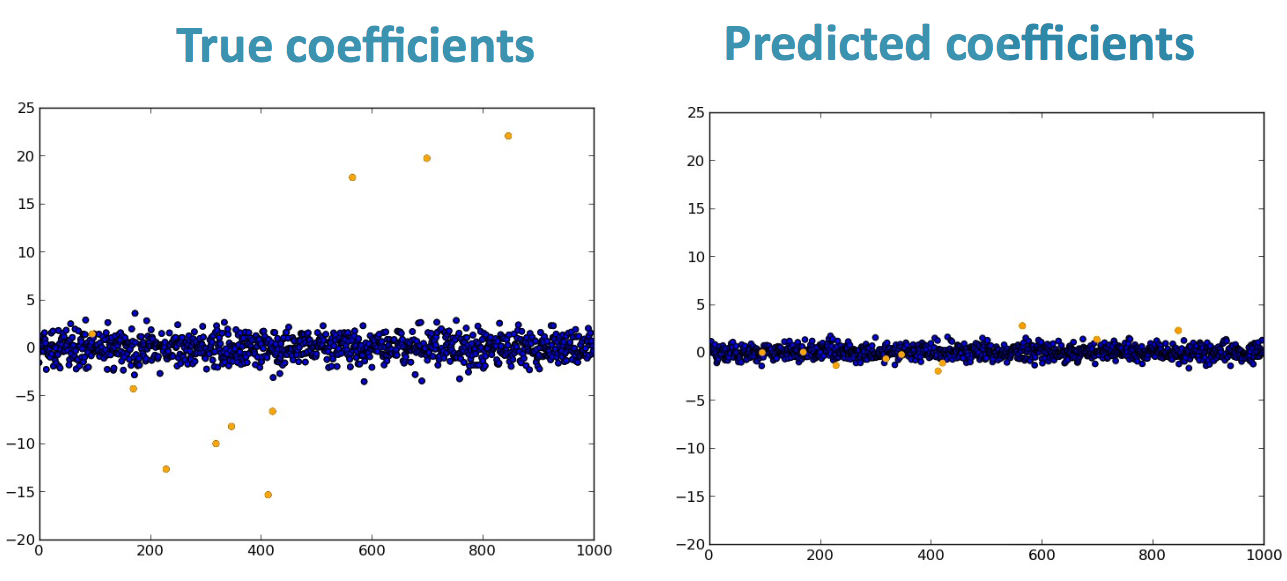
\includegraphics[scale = 0.3]{Figures/linear_regression_pseudoinverse.png}}
\caption{Example of weights obtained from linear regression when $X$ is not invertible, thus using the pseudo-inverse. On the left, the graph is showing the true coefficients of the vector $\beta$. On the right, the graph presents the predicted coefficients of the vector $\hat{\beta}$ obtained from linear regression.}
\label{LRPseudoInverse}
\end{figure}

\section{Regularization}
The Figure \ref{LRPseudoInverse} showed that the linear regression used all the features available to predict the outcome vector $y$. Yet, all the weights are very small. Thus, the solution is hard to interpret. Usually, we prefer having a small subset of features with strong weights. This is one of the advantages of regularization. Moreover, the more we have variables in our model, the more complex our model is. And, the more complex our model is, the more chances we have to overfit our data. Thus, we want to find a way to simplify our model.

 So, instead of minimizing only the sum of squared error, the idea of regularization is to minimize
 \[ \text{Sum of squared error} + \lambda \text{ prenalty on model complexity}.\]
Thus, when using regularization, the estimator is biased (if $\lambda \not = 0$). Yet, because the model will be less complex, we'll have a smaller variance. We're willing to accept a biased estimator in exchange for smaller variance. So, there's a tradeoff to make between bias and variance. $\lambda$ can be set by cross-validation. \label{CVlambda}

This method is also called \emph{shrinkage} in the context of linear regression. Indeed, this is going to shrink the weights of the model. Thus, the final model is simpler.

The following sections are presenting examples of regularization technique.

\subsection{Ridge regression}
\subsubsection{Ridge estimator}
Instead of minimizing our sum of squared error, ridge regression is aimed at minimizing $||y - X\beta||_2^2 + \lambda ||\beta||_2^2$. Thus, the ridge estimator is given by
\[ \hat{\beta}_\text{ridge} = \arg \min_\beta ||y - X\beta||_2^2 + \lambda ||\beta||_2^2. \]

\begin{thm} The ridge regression estimator is given by
\[ \hat{\beta}_\text{ridge} = (X^T X+ \lambda I)^{-1} X^T y. \]
\end{thm}

\begin{proof}
We consider the function $f$ defined by
\[ f(\beta) = ||y - X\beta||_2^2 + \lambda ||\beta||_2^2.\]
In order to minimize this function, we take its gradient.
\[ \nabla_{\beta}f(\beta) = -2X^T (y-X\beta) + 2\lambda \beta.\]
Then, $\beta_\text{ridge}$ is defined as $\nabla_{\beta}f(\beta_{\text{ridge}}) = 0$. Thus,
\[ (X^TX+\lambda I)\beta_\text{ridge} = X^T y.\]
If $\lambda > 0$, $(X^T X + \lambda I)$ is invertible, then
\[ \hat{\beta}_\text{ridge} = (X^T X+ \lambda I)^{-1} X^T y. \]
\end{proof}

\subsubsection{Solution path}
We've said in section \ref{CVlambda} that we can find the optimal value of $\lambda$ by cross-validation. We can compute solution paths (Figure \ref{SolutionPath}) that is a plot showing how the feature coefficient evolves when we decrease the value of $\lambda$. Indeed, when $\lambda = 0$, there's no regularization anymore. And, if $\lambda \gg 1$, we only want to minimize the model complexity. So, all coefficient are then equal to $0$. Then, on the Figure \ref{SolutionPath}, on the left hand, we start with the model in which all coefficients are equal to zero and we end, on the right hand, with the linear regression without any regularization model.

The vertical red line shows the value of $\lambda$ that was obtained by cross-validation. The goal is to choose the value of $\lambda$ that gives the best generalization on another set of data.
\begin{figure}[!h]
\centerline{
\includegraphics[scale = 0.3]{figures/solution_path.png}}
\caption{Ridge regression solution path}
\label{SolutionPath}
\end{figure}

\subsubsection{Standardization}
The goal of this section is to describe what will happen to our model if we multiply our features by a constant.
\begin{enumerate}
\item \textbf{Standard linear regression}~: Without any regularization, we multiply, in the data matrix $X$, the column $j$ by a real $c \not = 0$. So, 
\[\forall i \in [|0;n-1|], x_{ij} \to c x_{ij}.\]
Then, the corresponding weight $\beta_j$ is going to be divided by $c$.
\[ \beta_j \to \frac{1}{c} \beta_j.\]
Thus, the weight is different but the solution is similar.
\item \textbf{Ridge regression}~: When we multiply, in the data matrix $X$, the column $j$ by a real $c \not = 0$, we can't know what will happen because of the penalization term $\lambda \beta_j^2$. So, it's important to use standardized feature \emph{before} regularizing linear regression.
\end{enumerate}
\subsubsection{Advantages and drawbacks}
Finally,
\begin{enumerate}
\item \textbf{Advantages}~: Ridge regression has several advantages
\begin{itemize}
\item Correlated variables get similar weights.
\item Identical variables get identical weights.
\item An analytical solution is provided
\end{itemize}
\item \textbf{Drawbacks}~: And it also have drawbacks
\begin{itemize}
\item Ridge regression shrinks coefficients but does \emph{not} result in a sparse model. A model is sparse when many coefficient get a weight of $0$. Then, when a model is sparse, many coefficient can be eliminated from the model.
\end{itemize} 
\end{enumerate}

\end{document}